\documentclass[11pt, dvipsnames, usenames, aspectratio=169]{beamer}
\usepackage{amsmath, amsfonts, amscd, amssymb, amsthm, tikz,pgfplots}

\usepackage{caption}

\usetheme{Madrid}
\usepackage{CoeCollegeSPECIAL}
\usepackage{appendixnumberbeamer}

\bibliographystyle{aer}
\usepackage{natbib}

\setbeamersize{text margin left=10mm,text margin right=10mm} 

\title[Green Development within Urban Areas]{Commercial Green Development within Urban Environments: Theory \& Evidence}
\author{Evan Perry}
\date{August 31, 2021}

\begin{document}

\maketitlepage

\begin{frame}{Why Green Buildings? Why Spatially?}

\centering

\begin{tikzpicture}
\fill[rounded corners, crimson] (0,5) rectangle (3, 3) node[pos=.5, white]{\textbf{Scope}};
\fill[rounded corners, gold] (3.5,5) rectangle (6.5, 3) node[pos=.5, white]{\textbf{Feasibility}};
\fill[rounded corners, teal] (7,5) rectangle (10, 3) node[pos=.5, white]{\textbf{Timing}};
\fill[rounded corners, plum] (10.5,5) rectangle (13.5, 3) node[pos=.5, white]{\textbf{Space}};
\draw[rounded corners, thick, white] (2,-1) rectangle (11.5, 2);
\end{tikzpicture}

\end{frame}

\addtocounter{framenumber}{-1}

\begin{frame}{Why Green Buildings? Why Spatially?}

\centering
\begin{tikzpicture}
\fill[rounded corners, crimson] (0,5) rectangle (3, 3) node[pos=.5, white]{\textbf{Scope}};
\fill[rounded corners, gold] (3.5,5) rectangle (6.5, 3) node[pos=.5, white]{\textbf{Feasibility}};
\fill[rounded corners, teal] (7,5) rectangle (10, 3) node[pos=.5, white]{\textbf{Timing}};
\fill[rounded corners, plum] (10.5,5) rectangle (13.5, 3) node[pos=.5, white]{\textbf{Space}};
\draw[thick, ->] (1.5, 3) -- (1.5, .5) -- (1.9, .5);
\draw[thick, ->] (5,3) -- (5,2.1);
\draw[thick, ->] (8.5, 3) -- (8.5, 2.1);
\draw[thick, ->] (12, 3) -- (12, .5) -- (11.6, .5);
\draw[rounded corners, thick] (2,-1) rectangle (11.5, 2) node[pos=.5, text width = 9cm]{\begin{enumerate}
	\item Commercial green development policy is \textcolor{crimson}{\textbf{important}}, \textbf{\textcolor{gold}{practical}}, and \textbf{\textcolor{teal}{timely}}
	\item Effective policy design requires a \textbf{\textcolor{plum}{spatial perspective}}
\end{enumerate}};
\end{tikzpicture}

\end{frame} \note{

\tiny
We should start by asking, why should we care about green buildings at all, and even then, why should we care about where they're located? The easy answer is climate change. Homes, offices,  schools, the buildings that most all our activity occurs in --  these account for about 30\% of all greenhouse gas emissions in the US. Getting to some scenario where we win the fight against climate change necessitates that we build greener.
\bigskip

Another important component here is the uniqueness of green buildings. Specifically, when pursuing green buildings, what we're really doing is making spaces more energy-efficient, and thus cost-efficient. Energy-efficiency policies can be a win-win situation. Owners or occupants pay less for energy, collectively we reduce greenhouse gas emissions. Historically, energy-efficiency focus policy has much easier to legislate than more punitive policies. Even though those punitive policies are incredibly important, these efficiency-based polices are more attainable for many policymakers. So there's this combination of a big problem and an accessible solution. \emph{We see that green buildings are a low hanging fruit for local policy makers interested in fighting climate change.}
\bigskip

I should also note that this isn't just for local policy makers: the American Jobs plan contains billions of dollars to support the development of green infrastructure, particularly green homes and commercial buildings. So this topic is really pretty timely for even national policy makers.
\bigskip

The second question here is a bit trickier: why should we care about where these green buildings are located within cities? Again there a few reasons why we should care about this. For instance, there might be equity concerns involved in the energy-transition and our adaption to climate change, or  there might be location specific attributes that inhibit firms or developers from building green real estate. Maybe most important though is this question of where we should target policy. Should local policy makers focus on place-based policies, where cities target specific neighborhoods for green development? Or do they focus on broader incentive programs? These are important questions for local policymakers trying to mitigate climate change in their communities, and national policymakers when allocating funds.

}


\begin{frame}{What Do We Do?}

\begin{columns}
\begin{column}{.48\textwidth}

\begin{enumerate}
	\item \textbf{Theory:} \textit{Create an economic model to describe commercial green development within a city}
	
	\vspace{1.5cm}
	\item \textbf{Evidence:} \textit{Use data to test the model's predictions}
\end{enumerate}

\end{column}
\begin{column}{.5\textwidth}\centering
\captionof{figure}{Green Commercial Buildings,\\ Des Moines}
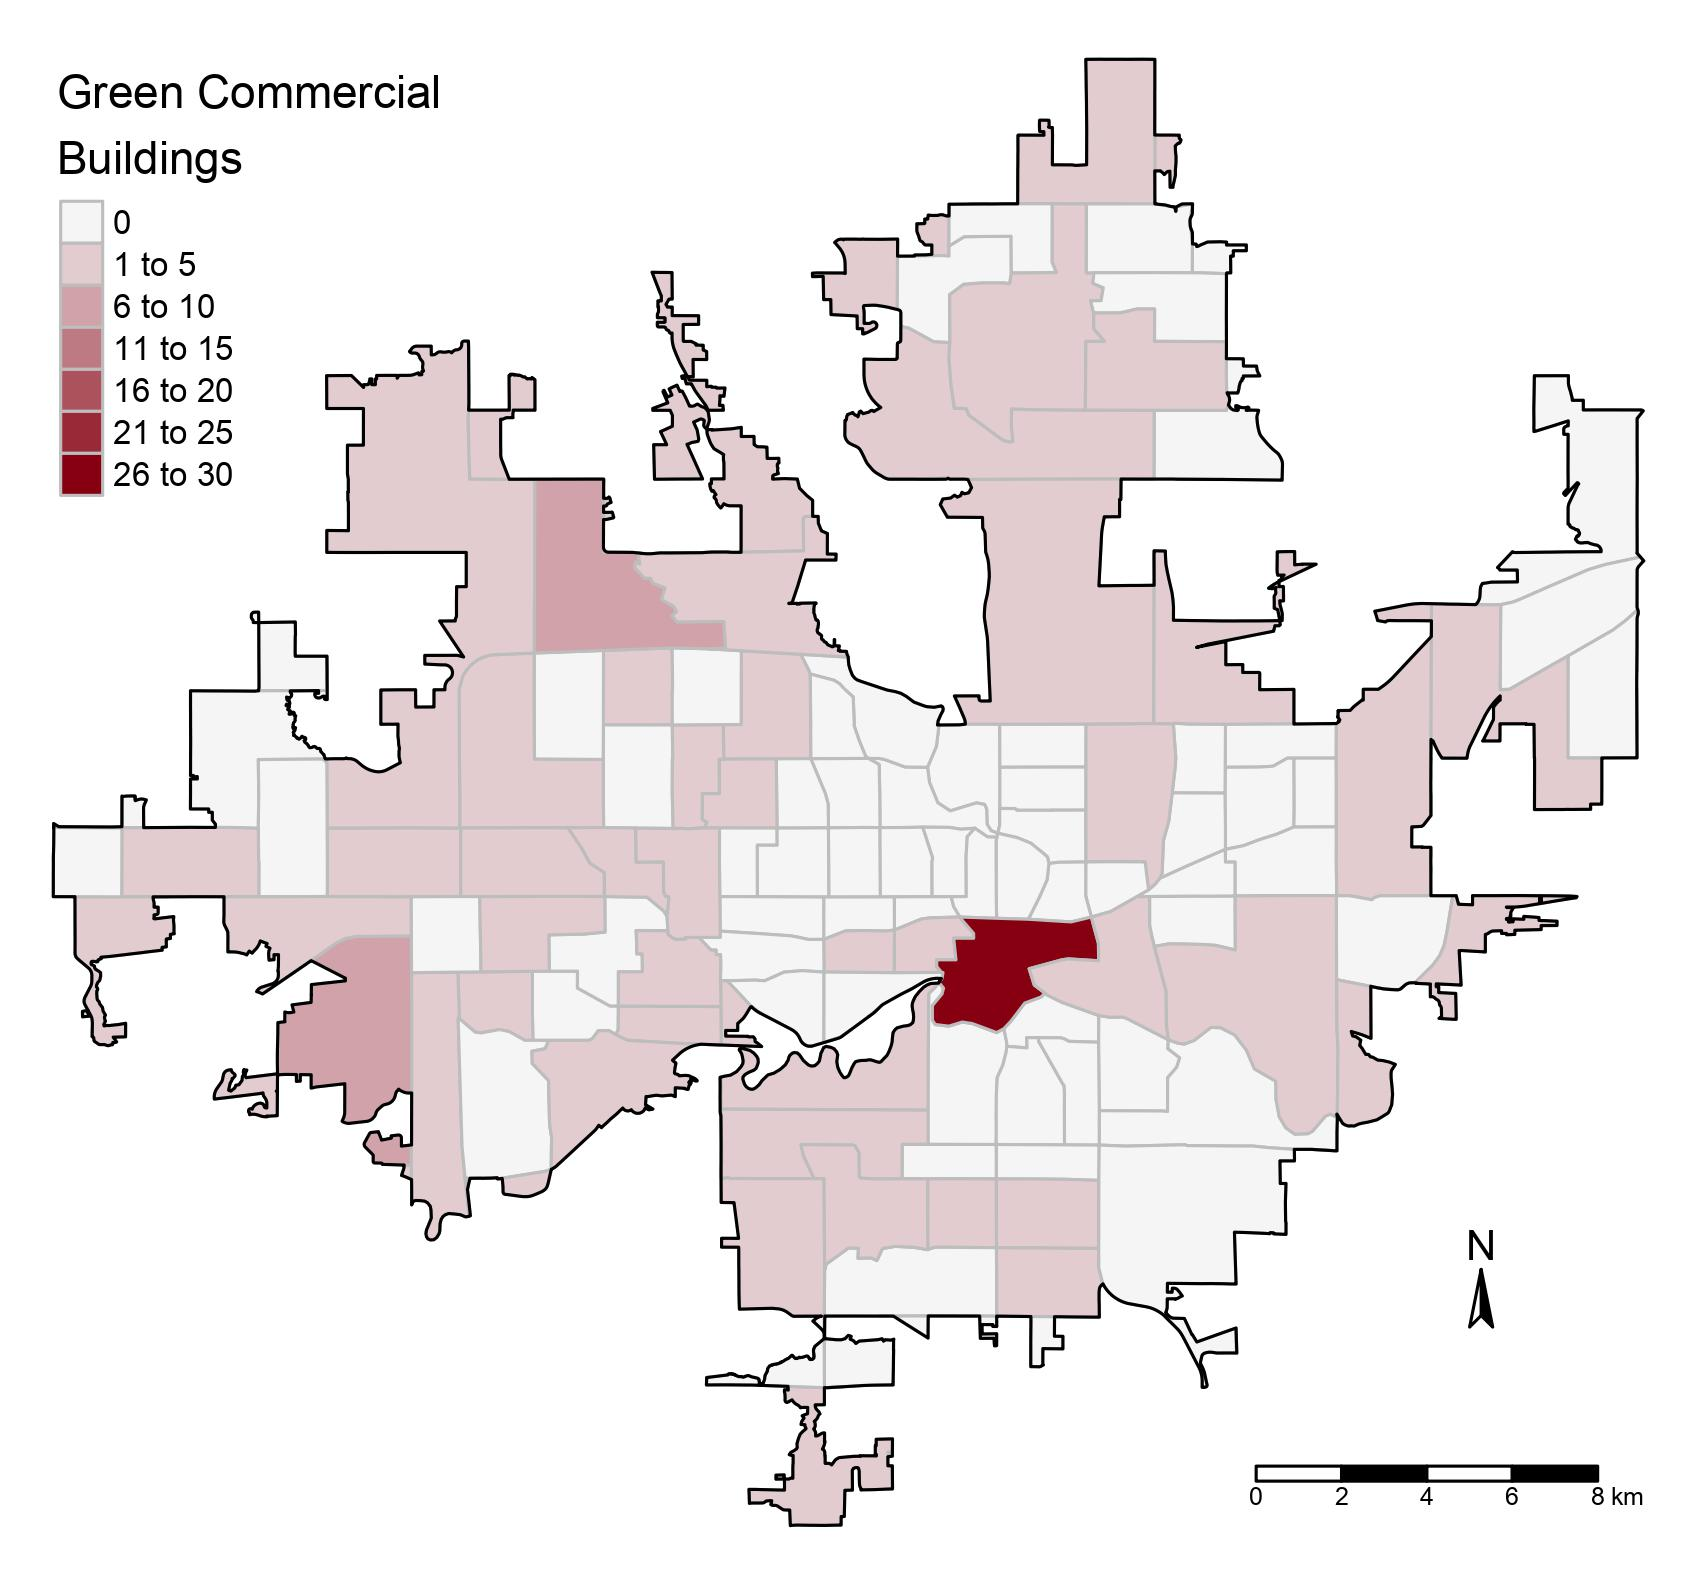
\includegraphics[width = 0.9\textwidth]{0001.jpg}
\end{column}
\end{columns}

\end{frame} \note{

Now this research doesn't answer these questions, but offers up a first-step towards these questions.

}

\begin{frame}{What Do We Find?}

\begin{enumerate}
	\item \textbf{Theory:} \textit{Forces that drive firms to locate in worker-dense neighborhoods also drive firms to prefer green real estate }
	
	\vfill
	\item \textbf{Evidence:} \textit{Worker-dense neighborhoods have more green real estate, even when controlling for the total number of workers}
\end{enumerate}

\end{frame}

%\begin{itemize}
%	\item The location and adoption decision are driven by similar industry characteristics 
%	
%	\vfill
%	\item Worker-dense neighborhoods will have a higher proportion of \textbf{\textcolor{EAPgreen}{green}} commercial real estate
%	
%	\vfill
%	\item Firm characteristics, not place characteristics, shape the adoption decision, so policy should focus on firms rather than places
%\end{itemize}

\begin{frame}
\Large\textcolor{crimson}{\textbf{Thank You}}
\end{frame}

\end{document}